
%% NB: conversation with Helen Hanlon - suggested that 10 years overlap period is not really enough o be capture sufficient natural variability (problem not to do with sample size - so including more grid cells doesnt really help with this).
% One idea would be to do an additional comparison over a longer period between aggregated daily values form 2.2km model and CEH-GEAR Daily.

% \documentclass[APA,STIX2COL]{WileyNJDv5}
\documentclass[APA,Times2COL]{WileyNJDv5}
\usepackage{geometry}
\usepackage[parfill]{parskip}
\usepackage{tabularx}
\usepackage{booktabs}
\usepackage{lscape}
\usepackage{enumitem}
\usepackage{subcaption}
\usepackage[demo]{graphicx}
% \usepackage[table,xcdraw]{xcolor}
% \usepackage{amsmath}
% Include numbering for {paragraph|}
% \setcounter{secnumdepth}{4}
% \usepackage{fontspec}
\usepackage{makecell}
\usepackage{todonotes}
\usepackage{afterpage}
\usepackage{tikz}
\usepackage{pgfplots}

\usepackage[export]{adjustbox}

\usepackage[utf8]{inputenc}
 
\usepackage[round]{natbib} % "round" will make the brackets like this: ()
% \bibliographystyle{ajs.bst}
\bibliographystyle{wileyNJD-APA.bst}

% \newcolumntype{C}[1]{>{\centering\arraybackslash}p{#1}}
\newcolumntype{L}[1]{>{\raggedright\let\newline\\\arraybackslash\hspace{0pt}}m{#1}}
\newcolumntype{C}[1]{>{\centering\let\newline\\\arraybackslash\hspace{0pt}}m{#1}}
\newcolumntype{R}[1]{>{\raggedleft\let\newline\\\arraybackslash\hspace{0pt}}m{#1}}

\newcommand{\subfigimg}[3][,]{%
 \setbox1=\hbox{\includegraphics[#1]{#3}}% Store image in box
 \leavevmode\rlap{\usebox1}% Print image
 \rlap{\hspace*{10pt}\raisebox{\dimexpr\ht1-2\baselineskip}{#2}}% Print label
 \phantom{\usebox1}% Insert appropriate spcing
}


% \setlength{\belowcaptionskip}{-10pt}
\graphicspath{{Figures/}} % Location of the graphics files

\title{\textbf{The sensitivity of urban pluvial flooding to the temporal distribution of rainfall within design storms}}
\date{}
% \author{Molly Asher}

\geometry{verbose,tmargin=1cm,bmargin=3cm,lmargin=2cm,rmargin=2cm}

\begin{document}
\maketitle
\vspace{-1.5cm}
% \pagestyle{empty}
\pagenumbering{arabic}

\section{Abstract}

% The risk posed globally by pluvial flooding to people and properties is growing due to rapid urbanisation, infrastructure development and intensification of rainfall due to climate change. Whilst tools to model pluvial flood hazard have also been rapidly developing, there remains a knowledge gap around the sensitivity of pluvial flooding to the temporal distribution of rainfall within design storms which are used to represent the extreme convective storm events that trigger it. 

The risk posed globally by pluvial flooding to people and properties is growing due to rapid urbanisation, infrastructure development and intensification of rainfall due to climate change. Whilst tools to model pluvial flood hazard have also been rapidly developing, there remains a knowledge gap around whether design storms used in modelling adequately represent the temporal distribution of rainfall within the extreme convective storms which drive flooding.  In the UK, the industry standard design storm considers rainfall events to always be symmetrical, and with a singular peak in intensity. Extensive study of UK extreme rainfall observations suggests that loading of rainfall towards the start or end of events is in fact more common. In the present study, the sensitivity of pluvial flood extent, hazard and timing to the shape of the rainfall profile in two urban catchments in the north of England is tested using fifteen realistic rainfall profiles derived from observed extremes. These realistic events are compared to idealised profiles, constructed through making systematic variations to the industry standard design storm profile to shift the single peak towards the start or end of the event. We demonstrate that for events with the same accumulated rainfall depth, both catchments show approximately a 15\% increase in the total flood affected area with the most back-loaded idealised profile compared to the most front-loaded, and a roughly 25\% increase with the most back-loaded observed profile compared to the most front-loaded. We conclude that the timing, as well as the magnitude, of the peak rainfall intensity in design storms plays a crucial role in determining the pluvial flood hazard. Consequently, failing to account for the observed variability in event profile shapes may result in substantial inaccuracies in the design of flood risk management solutions, leading to both underestimation and overestimation of the required measures. 

\section{Introduction}\label{sec:introduction}

Flooding is now the most frequently occurring and harmful natural hazard globally \citep{jenkins2018probabilistic, razavi2020anthropocene}. In England, pluvial flooding is the most widespread form of flooding, placing roughly 3.2 million properties at risk \citep{envagency2021}. Pluvial flooding - or surface water flooding as it is commonly known in the UK - occurs when the volume of rainfall exceeds the absorption capacity of the ground and the storm water drainage capacity \citep{archer_characterising_2015}. It generally occurs in urban settings which have a higher proportion of impermeable surfaces which preclude the natural processes that moderate floods in rural environments. The fast runoff and rapid response times in urban hydrology mean that pluvial flooding is more directly dependent than fluvial flooding on the characteristics of rainfall at smaller spatial and temporal scales \citep{ochoa2015impact, peleg2016partitioning}.

The influence of the temporal structure of rainfall has been a persistent question in hydrology for many years \citep{dawdy1969effect, singh1997effect, woods1999synthesis}. There has been substantial exploration into the temporal and spatial resolution of rainfall data required to faithfully represent the dynamics of storm events which influence urban hydrological processes. Temporal resolutions of between one and five minutes have been posited by several authors as a prerequisite for modelling certain processes \citep{schilling1991rainfall, einfalt2004towards, berne2013radar}. Much work has focused on providing data at this resolution through radar products \citep{einfalt2004towards, thorndahl2017weather, bruni2015sensitivity}, and stochastic rainfall generators, which produce sets of synthetic rainfall events which closely mimic the fine scale spatial and temporal structure of real rainfall events \citep{peleg2016partitioning, zhu2018impact, paschalis2014effects, gabellani2007propagation}. 

Although significant improvements have been made in these areas, it remains standard practice to use design storms in flood modelling. These are idealised rainfall events with greatly simplified characteristics \citep{butler_urban_2004}. They are advantageous as they avoid the need to model multiple individual historical rainfall events in a particular catchment, thereby reducing the computational burden, and they allow a standardised approach to assessing the impact of extreme rainfall \citep{marsalek1984design, balbastre2019comparison}. The total event accumulated rainfall depth is calculated through statistical analyses of historical rainfall data, and is generated for different durations and return periods. This rainfall depth is then distributed over time using a hyetograph which represents the time varying distribution of rainfall during a storm. The way in which the shape of the hyetograph is specified, and the impact of this on the resulting flood hazard, is the focus of this work.

There are a number of different approaches to specifying hyetographs. These are outlined in detail by \citet{chow1988applied}, \citet{veneziano1999best}, and \citet{balbastre2019comparison}, amongst others. The approaches can be loosely categorised as: observed (directly using temporal distributions from observed events); summary (generalising temporal distributions from observed events); geometric (using simple geometric shapes e.g. a triangle); stochastic (utilising stochastic rainfall models); or IDF curve-based methods (using rainfall characteristics from IDF (intensity duration frequency) curves alongside simple distribution shapes). 

In the UK, the industry standard approach to flood hazard modelling is to use one of two design hyetographs specified in the Flood Estimation Handbook (FEH) \citep{faulkner1999}. The FEH hyetographs are both symmetrical with a central peak in intensity, and bear a close similarity to the Chicago Design storm which is widely applied in other countries \citep{keifer1957synthetic, watt2013critical, yang2020linking}. The FEH profiles are to be applied regardless of the event duration or return period; with a summer profile, which is more sharply peaked, advised for use in urban areas, and a winter profile, which has a more shallow peak, recommended for rural catchments \citep{faulkner1999}. The FEH profiles are best described as summary hyetographs, and were derived by study and generalisation of just 80 summer (May to October) and 32 winter (November to April) storms of 24-hour duration occurring between 1961 and 1970. The generalisation process is described in detail by \citet{villalobos2023towards}. Importantly, in addition to the stages typical of generating summary hyetographs, the peak of each event is also shifted to the centre. This ensures that when summary profiles are derived from averaging across multiple observed rainstorms, there is always a temporally central peak in intensity. Whilst much of the flood estimation methods associated with the FEH have been updated more recently, the hyetographs have not been revised in the last fifty years. 

Recent research indicates that the FEH hyetographs are not representative of the true variety in the timing of peak intensity in observed storms. A set of $\sim$70,000 UK independent rainstorms ranging from sub-hourly to daily durations were identified by \citet{villalobos2023creation} using a new storm identification algorithm. These storms were used to trial an alternative approach to deriving summary hyetographs which removes the centering step applied in the FEH methodology. Rather, the positioning of the peak is made fundamental to the hyetograph classification, with profiles classed as front-loaded, centred or back-loaded. Importantly, \citet{villalobos2023towards} find that just 23\% of the observed storms have a central peak in intensity. This provides evidence that the majority of UK extreme storms are fundamentally different to design storms produced with the FEH hyetographs, and calls into question the validity of their continued application in UK flood modelling approaches. 

There is an inherent implication in the recognition of the sensitivity of urban hydrological models to the temporal resolution of rainfall used in continuous simulations, that the temporal distribution of rainfall in design storms must also influence the catchment response. A number of studies have also explicitly tested this. An early study by \citet{lambourne1987model} compared the peaks and volumes of runoff produced by four simple geometric design storm shapes in an urban Dutch catchment. \citet{nguyen2002rainfall} assessed the runoff peaks and volumes produced by seven commonly used design storms in Canada; \citet{balbastre2019comparison} investigated the hydrographs produced by eleven widely applied design storms for a rainfall-runoff model of an urban catchment in Valencia; \citet{krvavica2020evaluation} compare the performance of six design storms against two real rainfall events; \citet{hettiarachchi2018increase} apply six temporal patterns frequently used in the USA, for a model of an urban catchment in Minnesota; and \citet{li2021case} and \citet{bezak2018impact} produce a variety of hyetographs for Seoul and Slovakia, respectively, using Huff curves which are based on the quartile of the event in which most rainfall occurs \citep{yin2016intra}.

This existing research on the impact of the temporal distribution of rainfall in design storms on flood risk leaves two notable gaps. First, while studies applying idealised profiles have tested a variety of simple, summary temporal patterns, they have often failed to conduct systematic adjustments to these profiles to assess the consequences of shifting the timing of the peak intensity. Second, there is an absence of research examining realistic observed rainfall profiles within the context of the UK. This paper builds on the work of \citet{villalobos2023towards} to provide evidence on the sensitivity of urban hydrological response in a UK catchment to the distribution of rainfall in design profiles. Specifically, the aims of this paper are to use rain-on-grid flood modelling to test the sensitivity of flood extent, depth and timing in an urban catchment to: 

\begin{enumerate}
 \item The timing of the peak intensity in an idealised, single-peaked design storm. 
 \item The range of temporal distributions in physically realistic hyetographs, and to quantify how these outcomes differ from using a single-peaked design storm. 
\end{enumerate}

\begin{figure*}[htbp!]
\centering
\begin{subfigure}[b]{.65\textwidth}
\includegraphics[width=\linewidth]{Figs/Catchment/new_inset.png}\llap{
 \parbox[b]{4.3in}{(\textbf{a})\\\rule{0ex}{3.45in}}}\llap{
 \parbox[b]{1.5in}{(\textbf{b})\\\rule{0ex}{3.45in}}}
\end{subfigure}\qquad
\begin{subfigure}[b]{.3\textwidth}
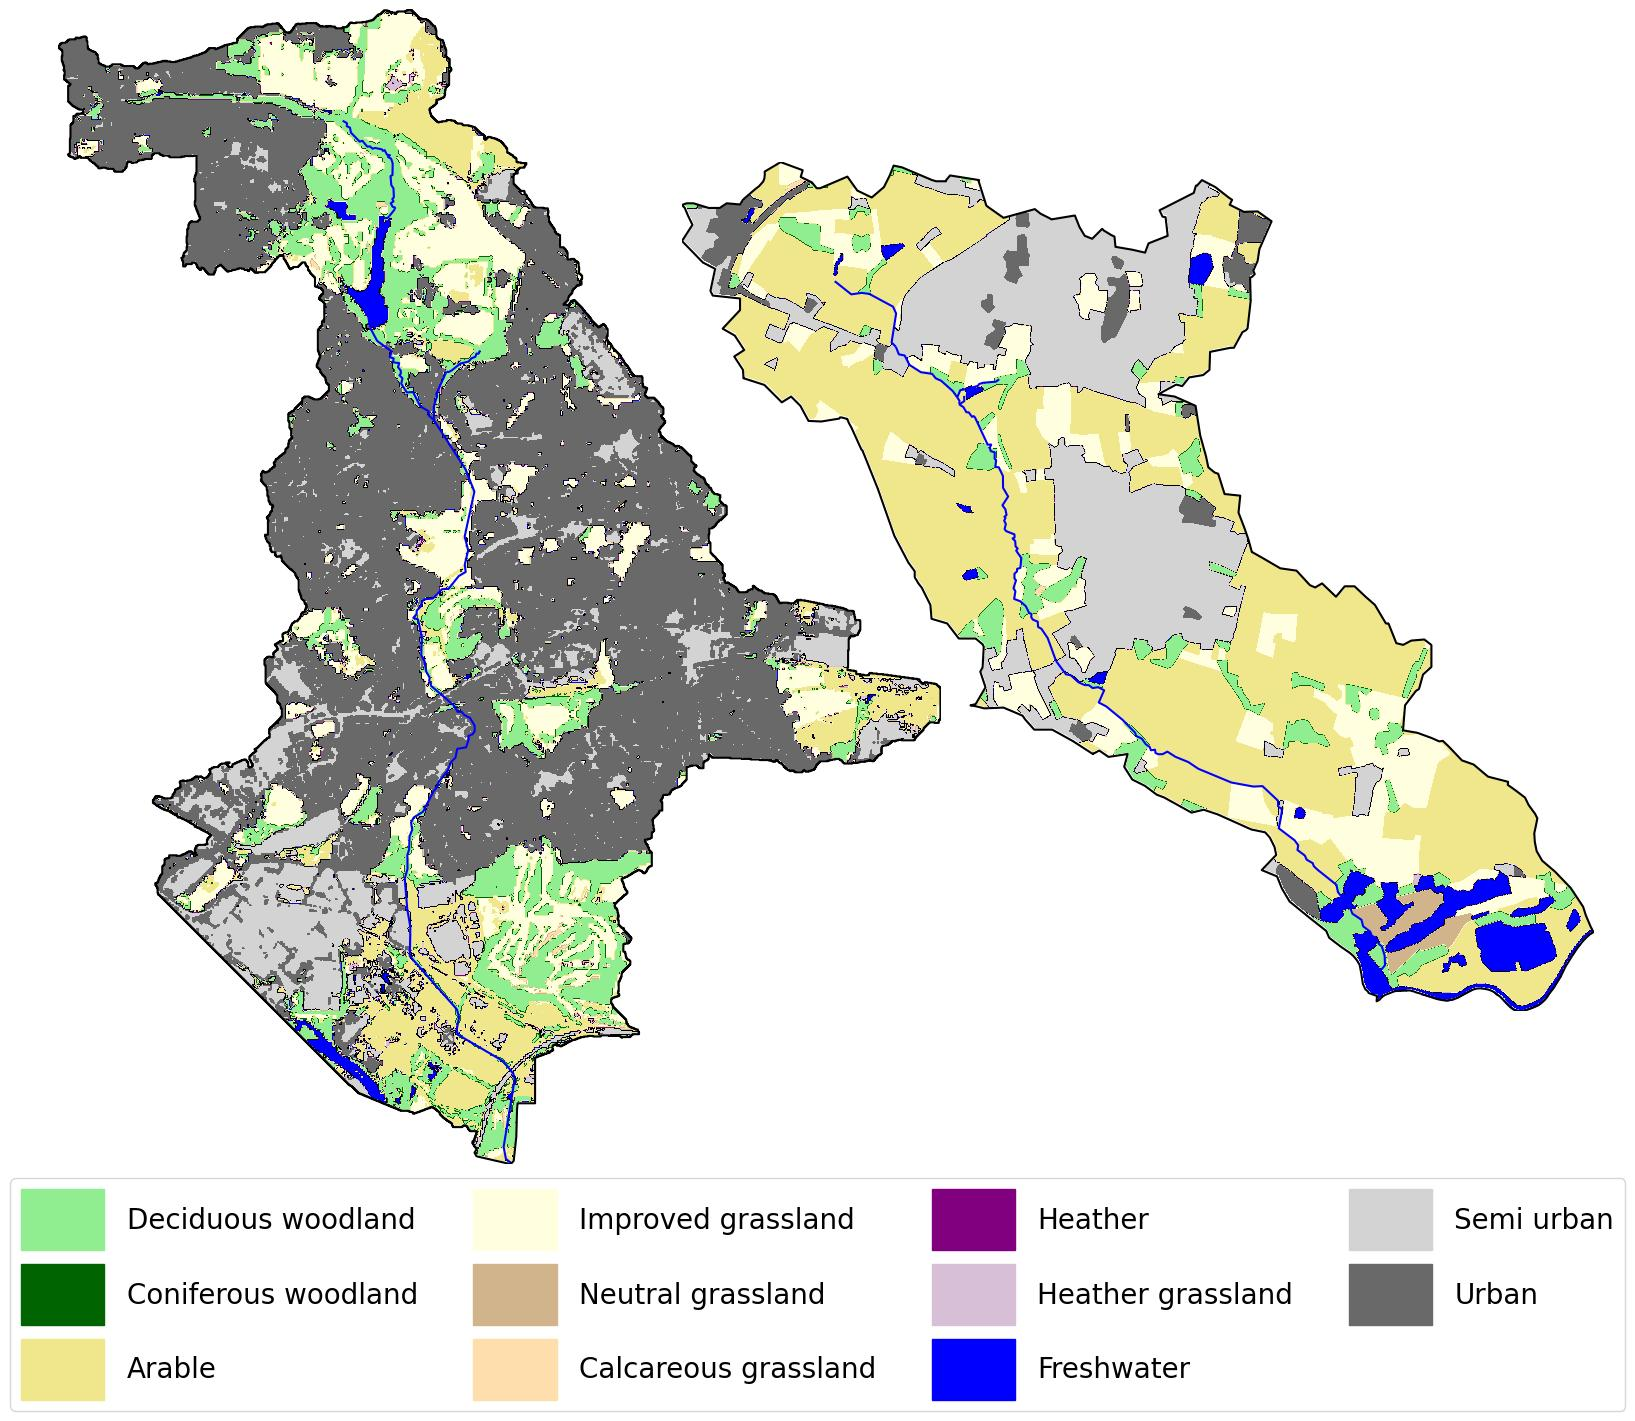
\includegraphics[width=0.99\textwidth]{Figs/Catchment/LandCover_BothCatchments.jpg}\llap{
 \parbox[b]{2.2in}{(\textbf{c})\\\rule{0ex}{1.6in}}}
% \vspace{2ex}
 \newline
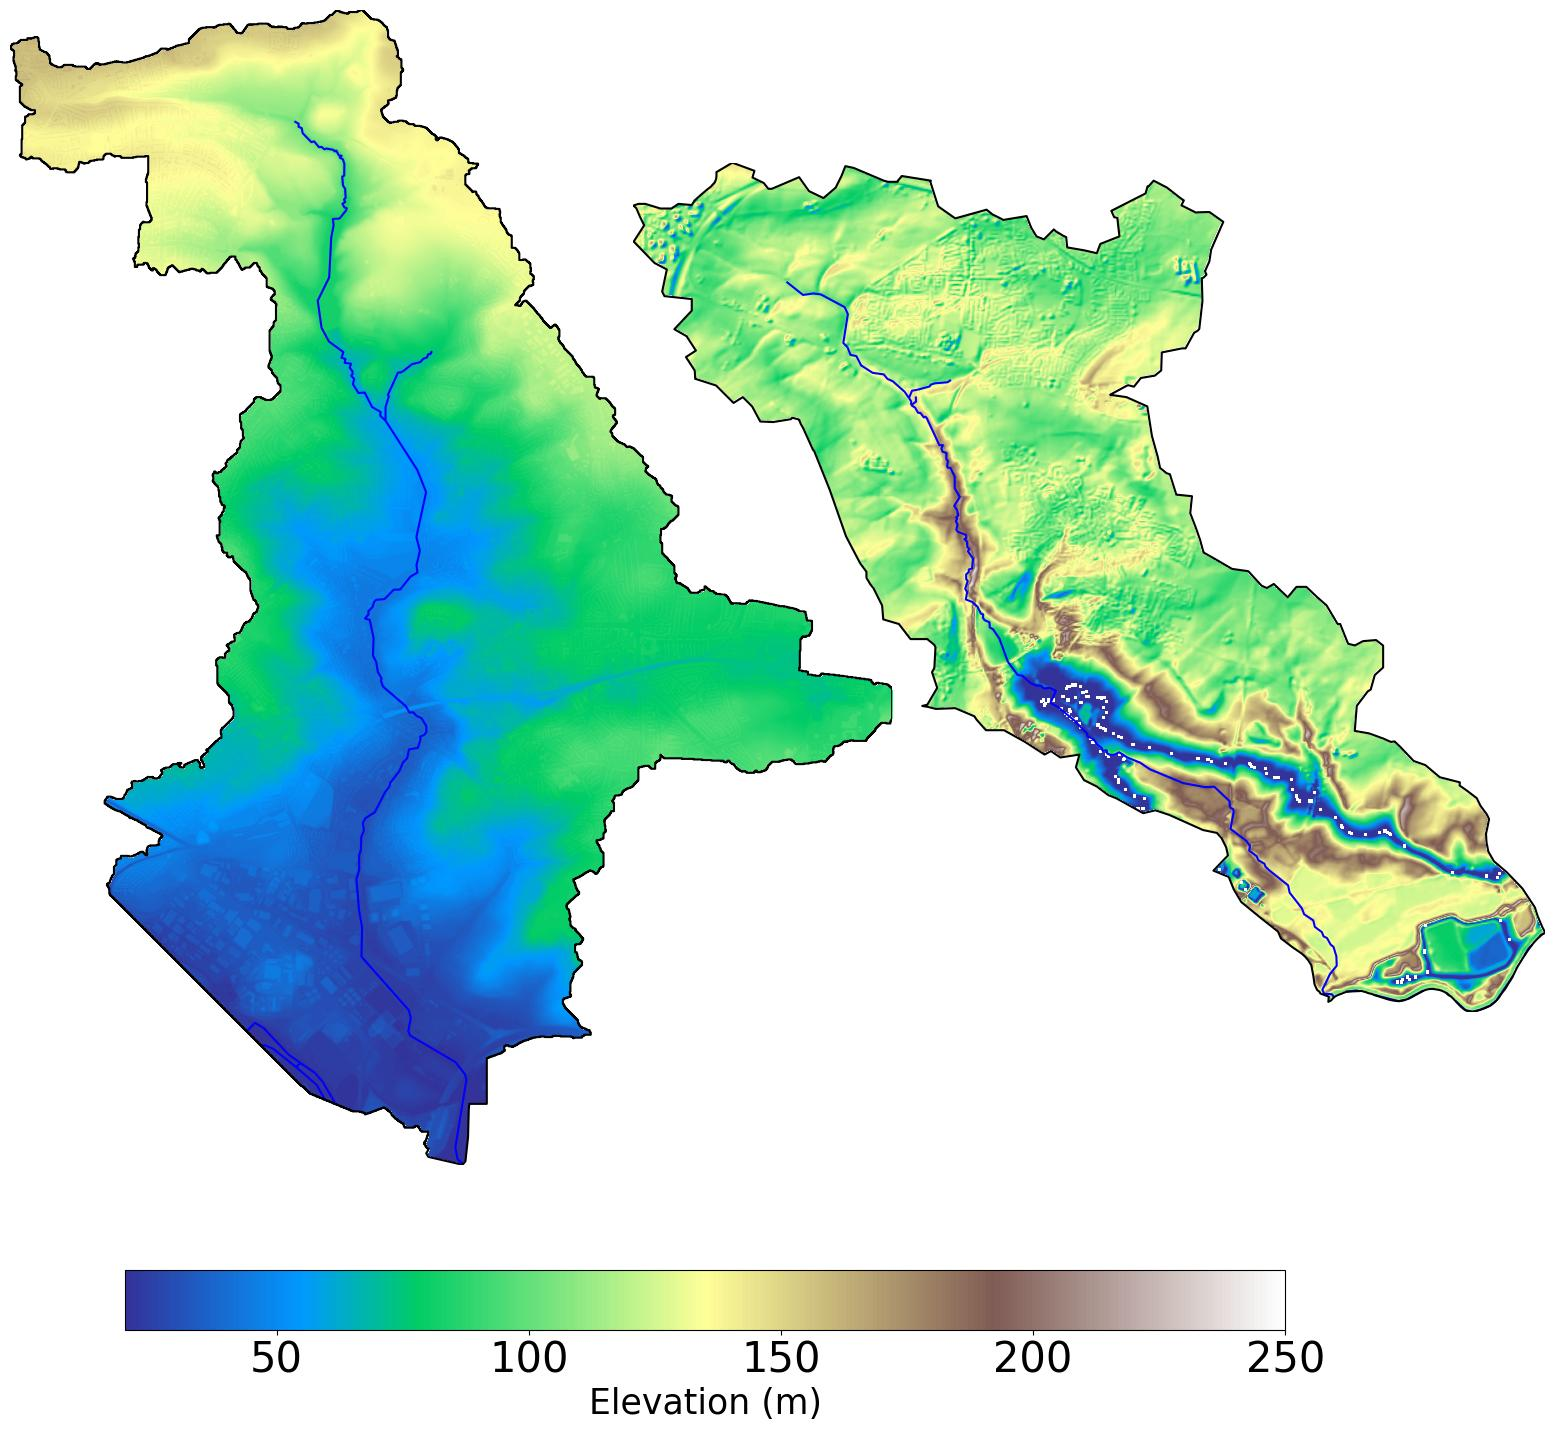
\includegraphics[width=0.99\textwidth]{Figs/Catchment/Terrain_BothCatchments.jpg}\llap{
 \parbox[b]{2.2in}{(\textbf{d})\\\rule{0ex}{1.5in}}}
\end{subfigure}
\caption{Geographical details of Wyke Beck (left) and Lin Dyke (right) catchments, including the location in the wider Leeds area with the main watercourse marked (a), the location in the UK (b), land use (c) and topography (d)} \label{fig:catchments}
\end{figure*}

%Fatone - urban catchments, NOT design storms
%Dullo - not clear, find site specific distributions and compares these against SCS Type II curve, which is widely used in the US
% Maca - rural catchment
% Fadhel - small urban catchment in west Yorkshire, NOT design storms. Look at how storm fractions scale with temperature, and then apply the scalings to storms (from the gauge record, I thinkk)
% Wasko and Sharmer - not even sure why I've referenced this,
%lamborne and stepehenson - urbanised catchment. Compares 4 very simple geometric hyetograph shapes to each other to assess differences in output hydrographs
%nguyen - mentuons urban drainage design in soutern Quebec, evaluate 8 popular design storms
%peyron - typicla urban basins in QUebec, this work is a bit confusing because it references previous work (Peyron, 2001), and the Nguyen paper also basically repeats a lot of this paper. But basically, they tested commonly used design storms. They found that no storm was good at replicating both runoff and volume from a real storm. They then created their own profile optimised for their specific area. Nguyen ^^ then looks at somrthing to do with climate change. 
% balabste-soldevide - urban catchment, valecnia; 11 well-known design storms
% hetteriarich - urban catchment, use 6 patterns from NOAA atlas (becomes 18 as 3 different volumes are trialled). also looks at impact of temperature scaling
% li - urban, construct rainfall events using Huff method (they don't exactly describe this, but there is some way to make it laoded in different ways 50% Huff, 10% Huff etc, so they construct a load of events with different loadings). 
%ng urban catchment, try to interrogate whether design storm concept is flawed by (as I understand): identifying the sensitive parts of the drainage system and then testing how much they respond to differences in stochastic rainfall events
%bezak - uses different versions of huff curves and looks at outputs

\section{Methods}\label{sec:methods}
\subsection{The study catchments}\label{subsec:model:catchments}
Wyke Beck and Lin Dyke are two suburban catchments on the eastern edge of Leeds (Figure \ref{fig:catchments}a), in the north of England (Figure \ref{fig:catchments}b). Wyke Beck covers 33.6 km\textsuperscript{2}, and has a large (63\%) urban share, including numerous populous Leeds suburbs. It also includes a smaller proportion (36\%) of green spaces, such as woodland and parks, and a small (1\%) contribution from the permanent water in Waterloo Lake, to the north of the catchment, and Wyke Beck, a tributary of the river Aire (Figure \ref{fig:catchments}c). Lin Dyke covers 22.9 km\textsuperscript{2}, the majority (69\%) of the catchment is rural land uses, such as farmland and woodland, with a smaller proportion (27\%) made up of urban and suburban land uses around the settlements of Kippax and Garforth. The remainder of the catchment (4\%) is permanent water, which is primarily found in the wetlands in the downstream area of the catchment, which drain into the river Aire (Figure \ref{fig:catchments}c). Wyke Beck has higher elevations to the headwaters of the catchment in the north, whilst in Lin Dyke the highest elevations are either side of the water course in the southern reaches of the catchment (Figure \ref{fig:catchments}d). 

\subsection{The flood inundation model}\label{subsec:model:catchments}

A 2D hydraulic rain-on-grid model is run in Hec-Ras model software (v6.4.1) using the 2D unsteady diffusion wave equation set \citep{brunner2016hec}. Hec-Ras has been used in a multitude of pluvial flood modelling studies, (e.g. \citet{costabile2021hec, yalcin2020assessing, singh2023drainage, rangari2019assessment}). Rain-on-grid modelling applies a rainfall input to each grid cell and simulates the movement of this water overland. Topography is defined with a Digital Elevation Model (DEM) and determines flow pathways and water ponding locations. Rain-on-grid modelling is a widely accepted approach to modelling pluvial flooding and was applied in the production of the Risk of Flooding From Surface Water (RoFSW) map \citep{envagency2019}. Despite this, there are some limitations to rain-on-grid modelling. In particular, it is common practice to not explicitly represent urban drainage and infiltration, and instead to reduce rainfall rates before applying them to the model in order to approximate these losses. The impact of this on our ability to assess the impact of the temporal profile on flood hazard is discussed in Section \ref{sec:discussion}.
% maybe add a sentence about more specifically that we aren't reying to improve the modelling process but that it has implications for our understanding of the rainfall processes

Existing flood models are used for both Lin Dyke \citep{beadle2021} and Wyke Beck \citep{singh2023drainage} catchments. The land use data for Lin Dyke is the UK CEH 2019 Land Cover Map \citep{morton2020land} and the OS MasterMap for Wyke Beck. Both models use a `bare earth' LiDAR DEM, at a resolution of 1m for Lin Dyke and 2m for Wyke Beck \citep{envagency2021}. Buildings alter surface runoff routes, and the DEM is adjusted by raising the terrain within building footprints to roof height using OS MasterMap data. Further adjustments are made to the DEM to ensure that hydraulic structures, such as bridges and culverts, are not unrealistically blocking the flow completely \citep{beadle2021, singh2023drainage, houston2011pluvial, wang2018integrated}). 

% reference for stampling on building: leandro2016step

The model is run for a total of 70 hours to ensure that the hydrological processes happening in the catchment after the storm are adequately captured. The model uses a variable time step, automatically adjusting it to maintain a Courant value within the range of 0.75 to 2. This adherence to the Courant condition ensures the stability of the simulation, with reliable and accurate results associated with a Courant value as close to 1 as possible \citep{rangari2019assessment}.

% Total rainfall depths for each rainfall probability / storm duration
% were scaled across a standardised storm profile to produce design
% hyetographs. Two standard profiles are typically recommended in
% the Flood Estimation Handbook: a 75% winter profile, for rural
% catchments, and a 50% summer profile, for urban catchments.
% The summer profile is more peaked than the winter profile, because
% of the prevalence of intense convective storms during the summer,
% so the intensity is greater in the middle of the storm. The summer
% profile is more likely to be critical for surface water flooding?


\subsection{The rainfall data}\label{sec:rainfalldata}
%The hyetograph of a rain for modeling a cloud burst scenario in Sweden is a combination
% of both frontal and convective storms or MCSs. The rising and falling limb located around
% an identifiable peak is usually the convective part, see figure 15 in section 4.3.5. 

Pluvial flooding is associated with short duration, convective rainfall events \citep{rudd2020investigating}. A six hour duration was chosen for this study as it has been shown to be the critical duration for Lin Dyke \citep{beadle2021}, i.e. the duration producing the highest peak flows \citep{daviescritical}. Although six hours perhaps seems long for a summertime convective event, this duration allows for a period of lighter rainfall either side of a convective peak. We modelled a 1-in-100 year return period event. As the middle of three options modelled in the RoFSW map \citep{envagency2019} we considered it a representative example of a moderately extreme scenario. 

Design storm profiles are required to translate this accumulated rainfall depth into the hyetographs which form the rainfall input to the flood model. We produce hyetographs using three different methods: (1) using the FEH standard summer profile (e.g. black line, Figure \ref{fig:profiles}a and b). This establishes a baseline - or standard - assessment of flood hazard in the catchments; (2) altering the FEH profile to shift its peak towards the start or end of the event, but conserving its shape and peak magnitude. This tests the impact of the timing of the peak on flood hazard in isolation from the confounding effects of peak magnitude (Figure \ref{fig:profiles}a); (3) using summary profiles produced from observed extremes. This quantifies the differences in flood hazard arising from the range of temporal distributions, and accompanying variations in peak magnitude, expected to be found amongst UK extreme rainfall events of this duration (Figure \ref{fig:profiles}b). Further details on the construction of each set of profiles is given below. In each case, the profile is produced for a six hour, 1-in-100 year event with an accumulated rainfall depth of 59.29mm for Lin Dyke and 59.25mm for Wyke Beck. This is calculated from the FEH web service which provides accumulated rainfall depths associated with specific durations and return periods for UK catchments.

\subsubsection{FEH profile}\label{subsubsec:feh}
The Revitalised Flood Hydrograph model (ReFH2) software is used to generate the FEH summer design profile for our catchments \citep{kjeldsen2013modelling}.
% The process used by the FEH to construct the summer design profile is outlined in the FEH guidance \citep{kjeldsen2007revitalised}. We generate this profile for our catchments using the Revitalised Flood Hydrograph model (ReFH2) software \citep{kjeldsen2013modelling}. 

\subsubsection{Idealised profiles}\label{subsubsec:idealised}
We produce an approximated version of the FEH summer design profile based on the FEH guidance \citep{kjeldsen2007revitalised}. Further details are provided in Appendix A. Eight further idealised profiles are created by shifting the peak of this approximated FEH summer profile in time, but otherwise retaining the shape. Four versions are front-loaded (with the peak in intensity occurring during the first half of the event) and four are back-loaded (with the peak in intensity occurring during the second half of the event). The profiles are created through rescaling the time axis before and after the peak. For example, for a front-loaded event, the rainfall curve before the peak is compressed, and after the peak it is stretched. More details on profile construction are given in Appendix B.

\begingroup
\setlength\tabcolsep{0pt}
\renewcommand{\arraystretch}{1.5} % Default value: 1
\begin{table*}[h!]
\centering
\caption{Descriptions of idealised and observed profiles, and abbreviations used in text}
\begin{tabular}{C{3cm}C{8cm}C{3cm}C{3cm}} 
 \hline
 \textbf{Title} & \textbf{Description} & \textbf{Idealised Profiles} & \textbf{Observed Profiles} \\ [0.5ex] 
 \hline
 Very front-loaded & Max intensity occurs in first 20\% of storm duration & I1, I2 & O1, O8, O15\\
 Front-loaded & Max intensity occurs in second 20\% of storm duration & I3, I4 & O3, O11, O10 \\
 Centred & Max intensity occurs in middle 20\% of storm duration & I5 & O6, O9, O13\\
 Back-loaded & Max intensity occurs in second last 20\% of storm duration & I6, I7 & O2, O12, O14\\
 Very back-loaded & Max intensity occurs in last 20\% of storm duration & I8, I9 & O4, O5, O7\\[1ex] 
 \hline
\end{tabular}
\label{table:profile_names}
\end{table*}
\endgroup

\subsubsection{Observed profiles}\label{subsubsec:observed}
We use fifteen temporal profiles identified through study of observed rainfall extremes between $\sim$two and six hours. \citet{villalobos2023towards} extracted rainfall events of these durations from a larger set of extremes of all durations. They performed a cluster analysis on the top 10\% (i.e. 1-in-10 year return period) events to capture the most common distribution profiles. The profiles describe the proportion of the total rainfall accumulated depth which falls within each of twelve time intervals for any event between $\sim$two and six hours. We construct profiles for a six hour duration, which is thus comprised of twelve time steps of 30 minutes each. The total rainfall accumulated depth falling in each 30 minute time step is assumed to fall at a constant rate, with each minute assigned a rainfall accumulated depth of 1/30th of the time step total. The time step total is calculated by multiplying the total event accumulated rainfall depth by the proportion of rainfall assigned to that time step. 


\begin{figure}[!t] 
% LEGEND
\begin{subfigure}[H]{\linewidth}
\flushright
\includegraphics[width=.95\linewidth,right]{Figs/Profiles/legend.png}
\end{subfigure}
% FIRST ROW
\begin{subfigure}[H]{\linewidth}
\includegraphics[width=\linewidth]{Figs/Profiles/Idealised_Observed_Profiles_LinDyke_prelossremoval.png}\llap{
 \parbox[b]{2.95in}{(\textbf{a})\\\rule{0ex}{0.98in}}}\llap{
 \parbox[b]{1.45in}{(\textbf{b})\\\rule{0ex}{0.98in}}}
\end{subfigure}
% SECOND ROW
\begin{subfigure}{\linewidth}
  \centering
  \includegraphics[width=\linewidth]{Figs/Profiles/Idealised_Observed_Profiles_LinDyke_postlossremoval.png}\llap{
 \parbox[b]{2.95in}{(\textbf{c})\\\rule{0ex}{1.08in}}}\llap{
 \parbox[b]{1.45in}{(\textbf{d})\\\rule{0ex}{1.08in}}}
\end{subfigure}
\caption{Hyetograph profiles for a six hour duration, 1-in-100 year return period event in the Lin Dyke catchment, including idealised profiles, pre-loss removal (a), observed profiles, pre-loss removal (b), idealised profiles, post-loss removal (c) and observed profiles, post-loss removal (d). The FEH summer profile is included in all plots in black. The profile classifications are explained further in Table \ref{table:profile_names}.} \label{fig:profiles} 
\end{figure}

\begingroup
\setlength\tabcolsep{0pt}
\renewcommand{\arraystretch}{1.5} % Default value: 1
\begin{table*}[h!]
\centering
\caption{Flood depth classification \citep{envagency2019}}
\begin{tabular}{C{3cm} C{14cm}} 
 \hline
 \textbf{Flood depth} & \textbf{Description} \\ [0.5ex] 
 \hline
 $<$0.1m & Considered to pose minimal hazard \\
 0.1-0.3m & Generally considered safe, likely to exceed kerb height \\
 0.3-0.6m & Unsafe for small vehicles, likely to cause property damage \\
 0.6-1.2m & Unsafe for all vehicles, and vulnerable groups, likely to cause property damage and exceed flood resilience measures level\\
 $>$1.2m & Unsafe for vehicles and people, buildings are vulnerable to failure \\
 [1ex] 
 \hline
\end{tabular}
\label{table:depth_cats}
\end{table*}

\setlength\tabcolsep{0pt}
\renewcommand{\arraystretch}{1.5} % Default value: 1
\begin{table*}[h!]
\centering
\caption{Velocity classification \citep{envagency2019}}
\begin{tabular}{C{3cm} C{14cm}} 
 \hline
 \textbf{Velocity} & \textbf{Description} \\ [0.5ex] 
 \hline
 $<$0.25 m s\textsuperscript{-1} & Considered essentially still \\
 0.25-0.5 m s\textsuperscript{-1} & Generally considered safe, could be a hazard to vehicles and vulnerable 
groups at deep depths \\
 0.50-2.0 m s\textsuperscript{-1} & Could be a hazard to vehicles and people at deep depths\\
 $>$2.0 m s\textsuperscript{-1} & Unsafe for vehicles and people, buildings are vulnerable to failure\\[1ex] 
 \hline
\end{tabular}
\label{table:velocity_cats}
\end{table*}

\setlength\tabcolsep{0pt}
\renewcommand{\arraystretch}{1.5} % Default value: 1
\begin{table*}[h!]
\centering
\caption{Hazard classification \citep{envagency2019} }
\begin{tabular}{C{3cm} C{4cm} C{10cm}} 
 \hline
 \textbf{Hazard class} & \textbf{Hazard Rating (HR)} & \textbf{Description} \\ [0.5ex] 
 \hline
 Low & $<$0.75 & Very low hazard - caution \\
 Moderate & 0.75 - 1.25 & Danger for some - includes children, the elderly and the infirm\\
 Significant & 1.25 - 2.0 & Danger for most - includes the general public \\
 Extreme & $>$2.0 & Danger for all - includes the emergency services \\
 \hline
\end{tabular}
\label{table:hazard_cats}
\end{table*}
\endgroup

\subsubsection{Loss removal}
%Mark comment; only if you don't use the inbuilt infiltration. You can drive it with gross rainfall and let it calculate spatially varied infiltration. However, it is has been standard FEH practice to drive these flood models with net rainfall (using ReFH2 to calculate losses) - so maybe just say following standard flood modelling practice....

The Hec-Ras models applied here do not explicitly model urban drainage, infiltration or evapotranspiration. Instead, the rainfall reduction approach is used, whereby a net rainfall input, with losses already subtracted, is applied to the catchment. The rainfall reduction approach is standard practice in pluvial flood modelling and was applied in the national RoSWF map \citep{envagency2019}, amongst other surface water flood modelling studies \citep{chen2009pluvial,chang2015novel, henonin2013real, wang2018integrated}. We use ReFH2 software to remove losses based on the physical catchment attributes. The mean summertime (June-July-August) daily rainfall for each catchment is specified as antecedent conditions for fifteen days prior to the event. For Lin Dyke this is 1.95mm and for Wyke Beck it is 2.02mm. We calculate the antecedent conditions using the 1km CEH-GEAR-1hr gridded observations \citep{lewis2019gridded} over the period 1990-2014 for the grid cells covering the catchment. ReFH2 has different methods for calculating losses in rural and urban areas. Our model applies rainfall in a spatially uniform manner. As the catchments are predominantly urban, we use ReFHs's urban loss removal model. This attenuates rainfall to 70\% to simulate infiltration, followed by the application of a fixed loss rate of 12mm/hr to account for the impact of urban drainage systems \citep{envagency2019}. 

\subsection{Flood classification}\label{subsec:model:data_analysis}
 % Only values from cells within the catchment boundary are considered. 
The maximum flood depth and velocity of flooding experienced in each cell across the whole model run time is exported from Hec-Ras as a raster (of the same resolution as the DEM). Detailed analysis is then conducted in Python. Only flood depths $>$ 0.1m are considered to constitute flooding, which is standard practice when assessing flood model results (e.g. \citet{houston2011pluvial, smith2019new}). In our modelling results we also aim to distinguish true flooding in areas which are usually dry, from areas of semi-permanent water, which are designed to be wet. We note that areas of permanent water, such as lakes or reservoirs, can appear as floodwaters in the results of Hec-Ras simulations due to how the software handles the interactions between river channels and adjacent floodplains. In Figure \ref{fig:flooded_area_spatial_BL}, areas which are classified in the land use data as fresh water are marked with hatching. This includes Waterloo Lake in the north of Wyke Beck catchment, and the substantial Fairburn Ings wetland region in the downstream area of Lin Dyke. In all of the analysis we exclude any areas identified as fresh water in the land use classification. Figure \ref{fig:flooded_area_spatial_BL} also reveals that the fresh water land use class does not cover the whole wetland area in Lin Dyke - perhaps because the wetlands are somewhat ephemeral - and also fails to capture some other areas of permanent water, such as some fishing ponds to the south of Kippax. Considering this, Figure \ref{fig:flooded_area_spatial_BL} also illustrates a boundary drawn for Lin Dyke which is used to additionally filter the results to ensure that none of these wetland areas are erroneously included in our results.

Our analysis includes calculation of the total flood affected area. This refers to the area in which flooding is experienced at some point during the model run time. Importantly, this whole area may not - and most likely will not - be all inundated at the same time. The next sections outline the approach taken to considering the flood depth, velocity and hazard categories of the flood waters.

\subsubsection{Flood depth and velocity categories}\label{sec:sec:depth_cat}
The flooded depths and velocities are considered in reference to the categories displayed in Table \ref{table:depth_cats} and Table \ref{table:velocity_cats} respectively. These have been defined by the \citet{envagency2019}, based on feedback from local flood authorities undertaken as part of the creation of the RoFSW map.

\subsubsection{Hazard classifications}\label{subsec:hazard}
The flood hazard rating ($HR$) is calculated using Equation \ref{eqn:hazard} as a function of flood depth ($D$), velocity ($V$) and a debris factor ($DF$). The debris factor is set, irrespective of the land use type, as 0.5 for depths $<=$ 0.25m, or 1 for depths $>$ 0.25m \citep{envagency2019}.

\begin{equation}
HR = D * (V +0.5) + DF
 \label{eqn:hazard}
\end{equation}

Table \ref{table:hazard_cats} provides thresholds for classifying this hazard rating according to the hazard it poses to people \citep{surendran2008supplementary}.


\begin{figure*}[h!]
  \centering
 \includegraphics[width=\textwidth]{Figs/SpatialPlots/WB_LD_05.png}\llap{
 \parbox[b]{6.85in}{(\textbf{a})\\\rule{0ex}{4.1in}}}\llap{
 \parbox[b]{4.25in}{(\textbf{b})\\\rule{0ex}{3.5in}}}\llap{
 \parbox[b]{5.50in}{\textbf{\textcolor{black}{\big{(1)}}}\\\rule{0ex}{2.0in}}}\llap{
 \parbox[b]{5.15in}{\textbf{\textcolor{black}{\big{(2)}}}\\\rule{0ex}{0.97in}}}\llap{
 \parbox[b]{2.5in}{\textbf{\textcolor{black}{\big{(4)}}}\\\rule{0ex}{1.9in}}}\llap{
 \parbox[b]{3.05in}{\textbf{\textcolor{black}{\big{(3)}}}\\\rule{0ex}{2.33in}}}\llap{
 \parbox[b]{1.84in}{\textbf{\textcolor{black}{\big{(5)}}}\\\rule{0ex}{1.39in}}}\llap{
 \parbox[b]{5.32in}{\textbf{\textcolor{black}{\small{Waterloo Lake}}}\\\rule{0ex}{3.5in}}}\llap{
 \parbox[b]{1.29in}{\textbf{\textcolor{black}{\small{Fairburn Ings Wetlands}}}\\\rule{0ex}{1.37in}}}\llap{
 \parbox[b]{2.55in}{\textbf{\textcolor{black}{\small{Fishing ponds}}\\\rule{0ex}{2.19in}}}}
 
\caption{The flooded area and depth from the most back-loaded observed profile (O5), for Wyke Beck (a) and Lin Dyke (b).  The flood depth categories correspond to those in Table \ref{table:depth_cats}. The watercourse is marked, and areas of permanent water according to the land cover classes in Section \ref{subsec:model:catchments} are marked with hatching. Areas of interest are marked with numbers and discussed in the text.}\label{fig:flooded_area_spatial_BL} 
\end{figure*}


\section{Results}\label{sec:results}

\subsection{Overview of catchment flooding}\label{subsec:overview}

The maximum flood depths associated with the most back-loaded observed profile leading to the most severe flooding (O5) are plotted for Wyke Beck (left) and Lin Dyke (right) in Figure \ref{fig:flooded_area_spatial_BL}. The depth categories correspond to those in Table 2. In both catchments, substantial inundated areas are observable around the track of the main watercourse. In Wyke Beck the most notable areas are: in the centre of the catchment, to the east of Harehills district (1); and around the industrial estate in the southern reaches of the catchment (2). In Lin Dyke, prominent inundated areas include locations to the south of Kippax, where the watercourse intersects a main road (3 and 4), and the area of wetlands in the lower catchment reaches (5). We are primarily interested in flooding in urban areas. In both catchments, flooding of streets and gardens can be observed in the urban areas.

\begin{figure*}[h!]
  \begin{subfigure}[b]{\textwidth}
    \centering
    \includegraphics[width=0.49\linewidth]{Figs/FloodedAreaBarCharts/LD_Notwater.PNG}\llap{
 \parbox[b]{2.95in}{(\textbf{a})\\\rule{0ex}{1.3in}}}\llap{
 \parbox[b]{1.45in}{(\textbf{b})\\\rule{0ex}{1.3in}}}
    \includegraphics[width=0.49\linewidth]{Figs/FloodedAreaBarCharts/WB_Notwater.PNG}\llap{
 \parbox[b]{2.95in}{(\textbf{c})\\\rule{0ex}{1.3in}}}\llap{
 \parbox[b]{1.45in}{(\textbf{d})\\\rule{0ex}{1.3in}}}
  \end{subfigure}
  % \vskip\baselineskip
  \begin{subfigure}[b]{\textwidth}
    \centering
    \includegraphics[width=0.49\linewidth]{Figs/FloodedAreaBarCharts/LD_Urban.PNG}\llap{
 \parbox[b]{2.95in}{(\textbf{e})\\\rule{0ex}{1.3in}}}\llap{
 \parbox[b]{1.45in}{(\textbf{f})\\\rule{0ex}{1.3in}}}
    \includegraphics[width=0.49\linewidth]{Figs/FloodedAreaBarCharts/WB_Urban.PNG}\llap{
 \parbox[b]{2.95in}{(\textbf{g})\\\rule{0ex}{1.3in}}}\llap{
 \parbox[b]{1.45in}{(\textbf{h})\\\rule{0ex}{1.3in}}}
    \centering
    \includegraphics[width=0.55\linewidth]{Figs/Profiles/legend.png}
  \end{subfigure}
\caption{The total area flooded (\textgreater 0.1m flood depth) at any point during the simulation, for areas which are not permanent water (a-d) and for urban areas (e-h). The percentage differences are shown relative to the centered profile (I5) for the idealised profile and relative to the FEH profile for the observed profiles.} \label{fig:total_flooded_area} 
\end{figure*}

\subsection{Changes to the total flood extent}\label{subsec:model}

The total flood affected area is displayed in Figure \ref{fig:total_flooded_area}. For each profile, the percentage differences are included relative to the centered profile (I5) for the idealised profiles and relative to the FEH profile for the observed profiles. Figures \ref{fig:total_flooded_area}a-d include the whole catchment minus areas of permanent water (as described in Section 3.3). They show that, for the idealised profiles, where the timing of the peak is shifted towards the end of the profile there is a consistent trend towards more extensive flooding in both Lin Dyke and Wyke Beck. The most front-loaded profile in both cases shows the most deviation from a centred profile, with 7.7\% less flooding in Lin Dyke and 6.8\% less in Wyke Beck. For the observed profiles, the trend is noisier. The centred profiles result in a smaller flooded area than the FEH profile, likely because of their lower peak magnitude (see Figure \ref{fig:profiles}d). In both catchments, the most back-loaded profile (O5) results in the most extensive flooding and a front-loaded profile (O8) results in the least extensive flooding; however, there are also front-loaded profiles that have a greater flooded area than some back-loaded profiles. This can be attributed to the considerable variation between these profiles in the magnitude, as well as the timing, of the peak intensity. 

Figures \ref{fig:total_flooded_area}e-h considers only flooding in areas which are classed as urban or semi-urban. We include this additional breakdown of results to rule out the possibility that the difference between the profiles is confined only to more rural parts of the catchment (e.g. fields) where flooding is less consequential. This demonstrates that, to the contrary, the differences between the sets of profiles are at least as large (or larger) for the urban areas than for the whole catchment. 

For the idealised profiles, across the whole of both catchments (except areas classed as permanent water) there is a $\sim$15\% increase in flood affected area from the most front-loaded profile to the most back-loaded. For the observed profiles, the difference is larger, with a $\sim$25\% increase from the most back-loaded profile to the front-loaded profile associated with the largest flooded affected area (Table \ref{table:depth_changes}). 

\subsection{Changes to the severity of flooding}\label{subsec:model}

The histograms in Figure \ref{fig:histograms} display the distribution of the total flood affected area in the catchment across the flood depth and velocity classes detailed in Section \ref{sec:sec:depth_cat}. For simplicity of interpretation, for both the idealised and observed profiles only the two scenarios which resulted in the greatest difference in flood extent are plotted (I9 and I1; and O8 and O5). 



Table \ref{table:depth_changes} also includes the proportion of the extra flood affected area in the most back-loaded profile, which falls within these depth and velocity categories. For both catchments and sets of profiles the majority of the extra flooding with a more back-loaded profile is relatively shallow. Around 60\% in Lin Dyke and 70\% in Wyke Beck of the additional flooding (for both sets of rainfall profiles) has a flood depth between 0.1 and 0.3m. Whilst these flood depths are generally not considered to pose much danger (see Table \ref{table:depth_cats}), it should be mentioned that they can still pose significant nuisance. Depths of $\sim$15cm are enough to reach the under body of a car and stall it \citep{ pregnolato2017impact}.  Depths over 10cm (the standard kerb height) begin to risk property damage \citep{moftakhari2018nuisance}. No more than 5\% of the additional flooding for either catchment or set of rainfall profiles reaches flood depths $>$1.2m. However, this equates to a significant extra area exposed to flood levels deemed as unsafe for all people and vehicles. 

In terms of velocity, for both rainfall profile options and both catchments, virtually none of the additional flooding is in the most severe category ($>$2 m s\textsuperscript{-1}). The split between the other categories varies, but between $\sim$20 and 30\% is always in the lowest category, which is virtually still and poses little risk, and between $\sim$70 and 80\% is in the medium risk categories.  

\begingroup
\setlength\tabcolsep{0pt}
\renewcommand{\arraystretch}{1.5} % Default value: 1
\begin{table*}[]
\caption{Increase in total flood affected area from the most front-loaded to the most back-loaded profile (I1 and I9 for idealised, O5 and O8 for observed). Includes the proportion of this extra flood affected area found in different depth and velocity categories. For instance, for the idealised profiles in Lin Dyke, the most back-loaded profile has 15\% more flood affected area than the most front-loaded, and 59\% of this extra area is between 0.1 and 0.3m in depth }\label{table:depth_changes}
\resizebox{\textwidth}{!}{
\begin{tabular}{C{5cm}C{3cm}C{3.5cm}C{3.5cm}C{3.5cm}C{3.5cm}} 
\hline
\multicolumn{1}{l}{\textbf{}} & \multicolumn{1}{l}{\textbf{}} & \multicolumn{2}{c}{Lin Dyke} & \multicolumn{2}{c}{Wyke Beck} \\ \hline
\multicolumn{1}{l}{\textbf{}} & \multicolumn{1}{l}{} & Idealised & Observed & Idealised & Observed \\ 
\hline
\topline
& & \multicolumn{4}{c}{\textbf{\begin{tabular}[c]{@{}c@{}}Increase in total flood affected area from most front-loaded to most back-loaded profile \end{tabular}}} \\ 
\Xhline{2\arrayrulewidth}
\multicolumn{1}{c}{Areal increase} & & 0.14 km\textsuperscript{2} & 0.22 km\textsuperscript{2} & 0.34 km\textsuperscript{2} & 0.61 km\textsuperscript{2}\\ 
\multicolumn{1}{c}{\% increase} & & 15\% & 25\% & 13\% & 24\% \\ 
% \hline \hline
\Xhline{2\arrayrulewidth}
& & \multicolumn{4}{c}{\textbf{\begin{tabular}[c]{@{}c@{}}The proportion of total increase in flood affected area from most front-loaded \\ to most back-loaded profile (shown above) in each of the flood depth and velocity categories\end{tabular}}} \\ \Xhline{2\arrayrulewidth}
\multirow{2}{*}{Flood depth category} & 0.1-0.3m & 59\% & 62\% & 72\% & 71\% \\
 & 0.3-0.6m & 17\% & 18\% & 18\% & 18\% \\
 & 0.6-1.2m & 19\% & 16\% & 8\% & 7\% \\ 
 & $>$1.2m & 4\% & 4\% & 2\% & 3\%\\
 \hline
\multirow{2}{*}{Velocity category} & 0.0-0.25 m s\textsuperscript{-1} & 32\% & 25\% & 20\% & 18\% \\
 & 0.25-0.5 m s\textsuperscript{-1} & 40\% & 47\% & 43\% & 50\% \\
 & 0.5 - 2.0  s\textsuperscript{-1} & 29\% & 27\% & 36\% & 32\% \\ 
 & $>$2.0 m s\textsuperscript{-1} & 0\% & 0\% & 1\% & 0\%\\
 \hline
\end{tabular}}
\end{table*}
\endgroup


\begin{figure}[!t] 
% FIRST ROW
\begin{subfigure}[H]{\linewidth}
\includegraphics[width=\linewidth]{Figs/Histograms/IP_Histograms_withoutwater.PNG}\llap{
 \parbox[b]{2.8in}{(\textbf{a})\\\rule{0ex}{1.68in}}}\llap{
 \parbox[b]{1.1in}{(\textbf{b})\\\rule{0ex}{1.68in}}}\llap{
 \parbox[b]{2.8in}{(\textbf{c})\\\rule{0ex}{0.75in}}}\llap{
 \parbox[b]{1.1in}{(\textbf{d})\\\rule{0ex}{0.75in}}}
\end{subfigure}
% SECOND ROW
\begin{subfigure}[H]{\linewidth}
\includegraphics[width=\linewidth]{Figs/Histograms/OP_Histograms_withoutwater.PNG}\llap{
 \parbox[b]{2.8in}{(\textbf{e})\\\rule{0ex}{1.68in}}}\llap{
 \parbox[b]{1.1in}{(\textbf{f})\\\rule{0ex}{1.68in}}}\llap{
 \parbox[b]{2.8in}{(\textbf{g})\\\rule{0ex}{0.75in}}}\llap{
 \parbox[b]{1.1in}{(\textbf{h})\\\rule{0ex}{0.75in}}}
\end{subfigure}
\caption{Histogram of the area in the flood depth and velocity categories defined in Section \ref{subsec:model:data_analysis} for idealised profiles (a-d) and observed profiles (e-h). In each case the most back-loaded profile and most front-loaded profiles are plotted} \label{fig:histograms} 
\end{figure}

Hazard class is a composite measure combining flood depth, velocity and a debris factor, with this debris factor relating to land use (see Section \ref{subsec:hazard}). In accordance with the results for depth and velocity, Figure \ref{fig:hazard_plots} illustrates that the increase in flood affected area in the back-loaded profiles occurs predominantly in the low hazard class across both catchments. There is a smaller increase in areas classified as moderately, significantly and extremely hazardous.

\begin{figure}[!t] 
% FIRST ROW
\begin{subfigure}[H]{\linewidth}
\includegraphics[width=\linewidth]{Figs/HazardPlots/IP_HazardCats_withoutwater.PNG}\llap{
 \parbox[b]{3.01in}{\textbf{(a)}\\\rule{0ex}{0.71in}}}\llap{
 \parbox[b]{1.37in}{\textbf{(b)}\\\rule{0ex}{0.71in}}}
\end{subfigure}
% SECOND ROW
\begin{subfigure}[H]{\linewidth}
\includegraphics[width=\linewidth]{Figs/HazardPlots/OP_HazardCats_withoutwater.PNG}\llap{
 \parbox[b]{3.01in}{\textbf{(c)}\\\rule{0ex}{0.71in}}}\llap{
 \parbox[b]{1.37in}{\textbf{(d)}\\\rule{0ex}{0.71in}}}
\end{subfigure}
 \caption{Number of flooded cells in each of the hazard classes defined in Section \ref{subsec:model:data_analysis} for idealised profiles (a,b) and observed profiles (c,d). In each case the most back-loaded profile and most front-loaded profiles are plotted}\label{fig:hazard_plots} 
\end{figure}


\subsection{Spatial changes to the flood extent and depth}\label{subsec:model}
\begin{figure*}[h!]
  \centering
 \includegraphics[width=\textwidth]{Figs/SpatialPlots/LD_Diff_all_leg3.png}\llap{
 \parbox[b]{2.48in}{{\textbf{(c)}}\\\rule{0ex}{1.25in}}}\llap{
 \parbox[b]{2.68in}{{\textbf{(d)}}\\\rule{0ex}{3.15in}}}\llap{
 \parbox[b]{6.28in}{{\textbf{(a)}}\\\rule{0ex}{3.15in}}}\llap{
 \parbox[b]{7.08in}{{\textbf{(b)}}\\\rule{0ex}{1.55in}}}\llap{
 \parbox[b]{3.8in}{{(1)}\\\rule{0ex}{0.45in}}}\llap{
 \parbox[b]{4.78in}{{(3)}\\\rule{0ex}{1.45in}}}\llap{
 \parbox[b]{4.25in}{{(2)}\\\rule{0ex}{1.22in}}}\llap{
 \parbox[b]{3.78in}{{(4)}\\\rule{0ex}{0.98in}}}
  \caption{The difference in flood depth between most front-loaded (O8) and most back-loaded (O5) observed profiles (e.g. O5-O8), across the whole of Lin Dyke (a), the Kippax urban area (b), the Garforth urban area (c) and a small section of Garforth (d). Areas of interest are marked with numbers and discussed in the text. }\label{fig:flooded_area_spatial_diff} 
\end{figure*}

Section \ref{subsec:model} establishes that the most back-loaded profile leads to the most extensive flooding. This extra flooding is comprised predominantly of incremental increases in the areas which experienced flooding in the more front-loaded profiles, rather than including any significant new areas which were not otherwise affected. An illustrative example of the areas which are subject to the largest changes in the maximum depth values between the most front-loaded and back-loaded observed profiles is given in Figure \ref{fig:flooded_area_spatial_diff} for Lin Dyke. The observed profiles are chosen for this demonstration because they exhibit the greatest difference in flood extent between the two extremes. In the vast majority of the catchment the back-loaded profile experiences deeper maximum flood depths than the front-loaded profile. The deeper flooding associated with the front-loaded profile, in the bottom area of wetlands (1), is likely an artefact of the duration of the model run time. Even after three days the model has not reached a steady state and water is still moving through the catchment. Consequently, for the back-loaded profile where the rainfall arrives later the depths in these storage areas in the lower reaches of the catchment are yet to reach the same levels as they do with the front-loaded profile. Given more time, we assume the depths in these areas would also be higher in the back-loaded profiles. 

The back-loaded profile has the most significant depth increases over the most front-loaded profile in the areas marked on the plot at 2, 3, and 4. The first of these locations is the fishing ponds marked in Figure \ref{fig:flooded_area_spatial_BL}. The latter two are at inundated areas which form at junctions between a major road and the watercourse. Notably, these ponds develop over fields and, therefore have less significant consequences. A more detailed look at the urban areas is provided for both Kippax (Figure \ref{fig:flooded_area_spatial_diff}b) and Garforth (Figure \ref{fig:flooded_area_spatial_diff}c), as well as an even more detailed look at the north-west of Garforth (Figure \ref{fig:flooded_area_spatial_diff}d). This shows that increases in flood depths of between 5 and 20cm are also commonly experienced in the urban areas which are vulnerable to flooding. These are not insignificant increases, and could make the difference between floods overtopping the kerb (which is usually around 10cm high) to cause property damage. 

\subsection{Changes to the simultaneously flooded extent over time}\label{subsec:flood_over_time}

Figure \ref{fig:flooded_area_over_time} illustrates the flooded extent at particular times during the course of the simulation. In agreement with Figure \ref{fig:total_flooded_area}, which includes the catchment area that experiences flooding at any time during the simulation, the most back-loaded profile is associated with the maximum flooded extents. For the idealised profiles in Lin Dyke (Wyke Beck), the maximum simultaneously flooded extent for the most front-loaded profile is only 91\% (84\%) the area of the most back-loaded profile. There is a more rapid onset of flooding with front-loaded profiles and they reach this maximum flooded extent 120 (130) minutes earlier in Lin Dyke (Wyke Beck). The difference in the timing of the peak in rainfall intensity between these two profiles is 288 minutes in both catchments (Figure \ref{fig:profiles}c). For the observed profiles in Lin Dyke (Wyke Beck), the maximum simultaneously flooded extent for the most front-loaded profile is only 89\% (86\%) of that of the most back-loaded profile. The difference in the timing of the maximum simultaneously flooded extent is even greater than with the idealised profiles, at 250 (300) minutes for Lin Dyke (Wyke Beck). A potential cause for this is that the difference in the timing of the peak in rainfall intensity between the most front-loaded and most back-loaded profile is even greater for the observed profiles at 331 minutes (Figure \ref{fig:profiles}d). 
% \textit{The difference in delay between the two catchments might be to do with size..?}

It is worth noting that the levelling off in the flooded area which we see in Figure \ref{fig:flooded_area_over_time} is to be expected for this kind of model. In pluvial flood modelling the focus is placed on accurately capturing the peak flood extent, which is predominantly what determines the flood risk. Capturing the tail end or the duration of the flooding would require significantly more advanced representation of the hydrological processes governing the movement, distribution, and properties of water over time. A lack of model connectivity prevents water draining and causes it to pond in an unrealistic manner. However, modelling the hydrology precisely would require extra - often difficult to access - data and come at a higher computational cost. Considering the limited benefits in terms of capturing the most relevant impacts of pluvial flooding, these costs are generally not deemed worthwhile.
% On the other hand, continuing loss occurs as a result of the processes of infltration and evapotranspiration, and they are assumed to proceed as far as the stormwater is available on the surface of the ground.

\begin{figure}[!t] 
\begin{subfigure}[H]{\linewidth}
\includegraphics[width=\linewidth]{Figs/FloodedAreaOverTime/legend_noFEH.png}
 \end{subfigure}
% FIRST ROW
\begin{subfigure}[H]{\linewidth}
\includegraphics[width=\linewidth]{Figs/FloodedAreaOverTime/LinDyke_FloodedAreaOverTime.PNG}\llap{
 \parbox[b]{2.98in}{(\textbf{a})\\\rule{0ex}{0.98in}}}\llap{
 \parbox[b]{1.45in}{(\textbf{b})\\\rule{0ex}{0.98in}}}
 \end{subfigure}
\begin{subfigure}[H]{\linewidth}
\includegraphics[width=\linewidth]{Figs/FloodedAreaOverTime/WykeBeck_FloodedAreaOverTime.PNG}\llap{
 \parbox[b]{2.98in}{(\textbf{c})\\\rule{0ex}{0.98in}}}\llap{
 \parbox[b]{1.45in}{(\textbf{d})\\\rule{0ex}{0.98in}}}
 \end{subfigure}
  \caption{The simultaneously flooded extent, plotted every ten minutes for the first eight hours and every two hours for the remainder of the model run time. For Lin Dyke catchment, idealised profiles (a), observed profiles (b); and Wyke Beck catchment, idealised profiles (c), observed profiles (d). The plots are cut off after 1400 minutes ($\sim$1 day) to allow the differences earlier in the process to be more clearly inspected. }\label{fig:flooded_area_over_time} 
\end{figure}

\section{Discussion and conclusions}\label{sec:discussion}

Storms are inherently unique phenomena characterised by a multitude of variables such as accumulated rainfall depth, duration, intensity, temporal and spatial patterns, and antecedent wetness conditions \citep{loveridge2018monte}. Attempting to represent the infinite range of possibilities associated with these variables in flood modelling would pose insurmountable computational challenges. Therefore, the design storm approach serves as a pragmatic solution, simplifying the modelling process to make it computationally feasible. Here we use a simulation model, following \citet{beven1989changing}, to explore the implications for pluvial flood modelling of the assumptions made in simplified design storms about the temporal structure of rainfall in real events. 

Our experiments with idealised profiles suggest that the assumption of a central peak in rainfall intensity in UK design storms neglects the presence of an important relationship between the timing of the peak rainfall intensity and the flood extent and severity. The construction of the FEH profile, similar to other hyetographs, primarily prioritises capturing the average rainstorm characteristics. \citet{villalobos2023towards} demonstrated that there is no true concept of an average storm, and we show here that by averaging across the actual variety in storms, differences are obscured which have a demonstrable impact on flood hazard. Specifically, we demonstrate a clear distinction between design storms with a later peak in intensity and those with earlier peaks. The systematic increase in the flooded area as the peak moves towards the end of the event could be attributable to a number of factors. Firstly, the prolonged period of light rainfall preceding the peak in back-loaded profiles may fill up small-scale storage elements within the landscape, such as small topographic depressions (e.g. puddles) or small drainage channels and roadside gutters \citep{bulti2020review}. Consequently, when the more intense rainfall arrives there is less storage available so water concentrates more quickly and levels of surface runoff may be higher. Furthermore, the cumulative effect of runoff from earlier stages of the event, coupled with the intensifying rainfall towards the end, can lead to a compounding effect, where floodwaters continue to rise, spreading over larger regions.

Testing with the fifteen observed profiles allows us to explore more generally the implications of the assumption that a single storm framework, in which the same design storm is always applied in all contexts, is adequate for representing flood risk in an urban catchment. \citet{villalobos2023towards} demonstrated the existence of a relationship between peak intensity and profile shape in observed extremes, with the highest intensities occurring only in very front-loaded or back-loaded events. The idealised profiles applied here, which include the same peak intensities across profile shapes, therefore lack physical realism. The observed profiles, however, represent the envelope of realistic combinations of timing and magnitudes of peak intensity that can be expected in UK extremes of this rarity and duration. The spread in output across these profiles (for instance, up to a $\sim$25\% difference in flooded area) suggest that the single storm framework may lead to a substantial misrepresentation of flood risk. There is a less consistent relationship between the timing of the peak intensity and the flood extent and severity as for the idealised profiles, likely because of the concurrent variation in the magnitude of the peak. Nonetheless, it remains notable that the profile with the smallest flooded area is associated with the most front-loaded rainfall intensity, while the profile resulting in the largest flooded area corresponds to a back-loaded pattern.

The modelling approach used here has some limitations. Standard pluvial flood hazard assessment methodologies are used, which apply a rainfall removal rate to represent the drainage capacity and infiltration. This simplified approach assumes that infiltration, and the influence of antecedent conditions, will occur in a spatially uniform manner. We propose that the disparity between the more pronounced flooding observed with the back-loaded profile and the milder flooding associated with the front-loaded profile could be even larger if the impacts of variations in permeable ground saturation and the filling of urban drainage systems during the early stages of the event were incorporated \citep{houston2011pluvial}.

The primary objective of this study is to examine the implications of simplifying the representation of the time-varying distribution of rainfall in design storms. The selected catchments are utilised not for the purpose of evaluating specific outcomes in these areas, but rather as tools to fulfill this objective. Catchment characteristics, particularly in complex urban watersheds, play a significant role in shaping hydrological responses \citep{singh1997effect, szelkag2022flood, ten2017role}. It is therefore important to address that these particular catchments possess unique attributes (size, orientation, elevation, urbanisation, topography etc) that likely influenced their responses. We present this research as an indicative example of the range of responses possible in a catchment purely from variations in rainfall temporal distribution, but note that the responses found here may not be representative of all catchments. Understanding of the interplay between catchment characteristics and rainfall variability is currently limited \citep{ten2017role}, and we support the need for more research into these complex relationships.

Even with further research, it is unlikely that a universal relationship between temporal rainfall variability and catchment characteristics will be uncovered. Applying a single storm framework therefore has evident shortcomings. \citet{villalobos2023towards} illustrate an evidence-based approach to deriving a suite of profiles which could replace the FEH profile. They also provide evidence of the most common hyetograph shapes found at different durations. If a single storm framework must be used, then we recommend that making an informed choice from these profiles, based on duration, could improve the accuracy of results. For instance, for very short duration storms, very front-loaded profiles have been shown to be the most common. Ideally, alternative approaches to a single-storm framework would be considered, such as ensemble modelling or Monte Carlo simulations \citep{nathan2003use}. An excellent example of this approach is found in the Australian Rainfall and Runoff (ARR) national guidance document for estimation of design floods in Australia \citep{ball2019australian}. In its most recent update the ARR recommends, instead of the previous single storm method, to use an ensemble of temporal patterns derived from extensive data and specific to location, duration and frequency. There are ten temporal patterns for each duration, ranging from ten minutes to seven days, for each of four return period bands and each of twelve regions. Consequently, flood modelling outcomes are more tailored to the specific characteristics of the rainstorm and region, while also providing a range or ensemble of potential forecast outcomes, each with equal probability, to better quantify forecast uncertainty. \citet{villalobos2023towards}'s profiles offer an opportunity to move towards a similar system in the UK, and we recommend exploring how to implement this effectively.

% These findings have profound implications for flood risk management, urban planning, and infrastructure design. The accurate representation of rainfall temporal distribution is not merely an academic concern but a critical consideration for safeguarding communities and properties. Our results emphasize that overlooking the temporal aspects of rainfall can lead to a significant underestimation of flood risks. Moreover, the distributed and relatively shallow nature of additional flooding with back-loaded profiles suggests that existing drainage systems and flood mitigation measures may need to be re-evaluated and adapted to accommodate such scenarios.

\section*{Appendix A: Approximation of FEH summer design profile}\label{sec:app_profiles}

The FEH summer design storm profile is approximated using the method outlined in the FEH guidance \citep{kjeldsen2007revitalised}. Equation \ref{eqn:fsr} is applied for a six hour duration, 1-in-100 year return period event (with an accumulated rainfall depth of 59.29mm for Lin Dyke; and 59.25mm for Wyke Beck, as described in Section \ref{sec:rainfalldata}), where the proportional depth of rain, $y$, falling in the temporal proportion, $x$, of the total duration, centered on the peak is given as:

\begin{equation}
\text{y} = \frac{1-a^{z}}{1-a}
 \label{eqn:fsr}
\end{equation}

where \textit{z} = $x^b$, and $a$ = 0.100 and $b$ = 0.815 for the summer profile. 

It is a known limitation of this formula that it gives unrealistically large values for the summer profile when a small timestep (i.e. a small value of $x$) is used. However, despite amendments being made to this formula since its initial publication, no supporting documentation of the implemented amendments are openly offered. Consequently, our approximation of the FEH rainfall curve has a slightly sharper and higher peak than that produced by ReFH2, and this presents a small limitation in our work. 

\section*{Appendix B: Idealised asymmetric rainfall profiles}\label{sec:app_profiles}

In order to calculate the rainfall rate for an idealised asymmetric rainfall peak, the location of the peak is changed, but otherwise the shape of the rainfall profile is kept the same. To achieve this, we must effectively rescale the time axis both before and after the peak: e.g., for a front-loaded event the rainfall curve before the peak is compressed, and the profile after the peak is stretched. 

The fraction of rainfall before the peak $f_*$ scales with the fraction of time before the peak $f_* = (t_{peak}-t_{start})/(t_{end}-t_{start})$. This is easy to see for a triangle-shaped rainfall profile, i.e. one that linearly increases and decreases in intensity before and after the peak, but also applies to our profiles.

We define a rescaled time $t_*$, which is given as
\begin{align*}
&t_*=(t-t_{peak})/(t_{peak}-t_{start}) \\ & \textrm{ when } t_{start} <t<t_{peak} \textrm{, in which case } -1<t_*<0, \\
&t_*=(t-t_{peak})/(t_{end}-t_{peak}) \\ & \textrm{ when } t_{peak} \leq t<t_{end} \textrm{, in which case } 0 \leq t_*<1. 
\end{align*}

As an example, the profile of $A/A_{total}$ for an event where $f_*=0.2$ is shown in figure \ref{fig:accprof}. Here, $A_{total}$ is the total rainfall accumulation over the event. 

\begin{figure}
\includegraphics[width=8cm]{tikz_accumulation.pdf}
\caption{Accumulated rainfall depth profile $A/A_{total}$ for an asymmetric (front-loaded) rainfall event where $f_*=0.2$.}
\label{fig:accprof}
\end{figure}

The accumulation at a given scaled time $t_*$ is given by the following equations, which are a generalisation of the FEH design storm profiles (the FEH design storm profiles correspond to $f_*=0.5$). 
\begin{align*}
A(t_*) = & A_{total}\left(f_*-f_* \frac{1-a^{(-t_*)^b}}{1-a} \right) \\ & \textrm{when } t_{start}<t<t_{peak}, \\
A(t_*) = & A_{total}\left(f_*+(1-f_*) \frac{1-a^{(t_*)^b}}{1-a} \right) \\\ & \textrm{when } t_{peak} \leq t<t_{end}.  
\end{align*}

The corresponding rainfall rate is calculated by numerically differentiating the accumulation curve on a minute-by-minute basis. Rainfall profiles for events with different values of $f_*$ are shown in Figure \ref{fig:profiles}a in the main text.

%%%%%%%%%%%%%%%%%%%%%%%%%%%%%%%%%%%%%%%%%%%%%%%%%%%%%%%%%%
% REFERENCES
%%%%%%%%%%%%%%%%%%%%%%%%%%%%%%%%%%%%%%%%%%%%%%%%%%%%%%%%%%
\newpage
\clearpage
\bibliography{Refs.bib}

\end{document}
